\documentclass[t, 10pt]{beamer}
%%\documentclass[t,handout]{beamer}

\usepackage{graphicx}
\usepackage{epsfig}
\usepackage{psfrag}
\usepackage[english]{babel}
\usepackage{color}
%Mathematics packages
\usepackage{amsmath}
\usepackage{mathrsfs}
\usepackage{amsfonts}

\usepackage{enumerate}


\graphicspath{{./images/}} % Figures path - used in graphicx

\selectcolormodel{cmyk}

\mode<presentation>

%THEMES - Please refer to these chapters in the beamer documentation.
% Presentation themes : Chapter 15
% Color themes : Chapter 17
% Font themes : Chapter 18


\usetheme{Pittsburgh}
\usecolortheme{orchid}
\usefonttheme{default}

%---------------------------Title frame definition------------------------------------- 

\title{Usage Management of Personal Medical Records}
\author [Chris]{Christopher Lamb, Pramod Jamkhedkar, and Gregory Heileman}
\institute[University of New Mexico]{
\inst {}Department of Electrical and Computer Engineering\\
University of New Mexico}
\date{Februrary 24, 2011}
\titlegraphic{
\begin{figure} 

\includegraphics[width = 7cm]{UNM}
\end{figure}}

% Delete this, if you do not want the table of contents to pop up at
% the beginning of each subsection:
%\AtBeginSubsection[]
%{
%  \begin{frame}<beamer>
%    \frametitle{Outline}
%     \tableofcontents[currentsection,currentsubsection]
%  \end{frame}
%}


\begin{document}

\begin{frame}
\titlepage
\end{frame}

% This command will make the logo appear on all frames excluding the title frame.
\logo {
\includegraphics[width = 2.5cm]{UNM}}

\begin{frame}
\frametitle{Outline}
\tableofcontents 
\end{frame}

\section{UNM Informatics}
\begin{frame}
\frametitle{Areas of Study}

Our group:
\begin{itemize}
\item \textit{UNM Informatics}: Information security, theory, and architectures; this work is specific to information security 
\item \textit{Usage Management}: Control of how an artifact is used, covering everything \textit{after} access as well as controlling access itself
\end{itemize}
\pause

\textit{Motivation}: We believe people should have control over their own information.  Or past motivation for DRM work was to provide content control to content creators.  Doing so provides incentive for innovation, and improves quality of life for individuals and society as a whole over time.  We believe Usage Management provides the same benefits, and should be unobtrusive.
\newline
\newline
This motivation holds in this domain as well.
\pause

Acronyms:
\begin{itemize}
\item \textit{UM}: Usage Management
\item \textit{PMR}: Personal Medical Record (this is also electronic, in this case)
\end{itemize}

\end{frame}

\section{Personal Medical Records}
\begin{frame}
\frametitle{UM and PMRs}

PMRs have certain attributes that aren't addressed well by current management systems:
\pause
\begin{itemize}
\item \textit{Mashable}
\pause
\item \textit{Controllable}
\pause
\item \textit{Available}
\end{itemize}
\pause

Usage Management of PMRs enables these things, providing fine-grained management of \textit{information contained in PMRs}
\newline
\pause

This opens new business models:
\pause
\begin{itemize}
\item \textit{Remote Access}
\pause
\item \textit{Monitoring}
\pause
\item \textit{Custom Care}
\pause
\item \textit{Data Marketplace}
\end{itemize}
\pause

But also new \textit{risks}.
 
\end{frame}

\section{UM Primer}
\begin{frame}
\frametitle{UM Primer - UM System}

Three basic things:
\begin{figure}
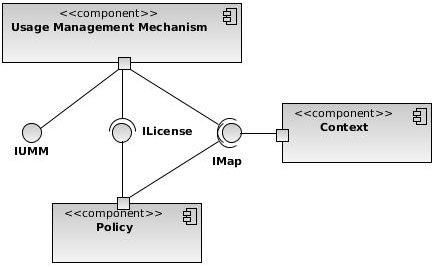
\includegraphics[width = 6cm]{Integrated}
\end{figure}

\begin{itemize}
\item \textit{Usage Management Mechanism}
\item \textit{Policy}
\item \textit{Context}
\end{itemize}

\end{frame}

\begin{frame}
\frametitle{UM Primer - Ontology}

Ontology of domain required to pull it all together
\begin{figure}
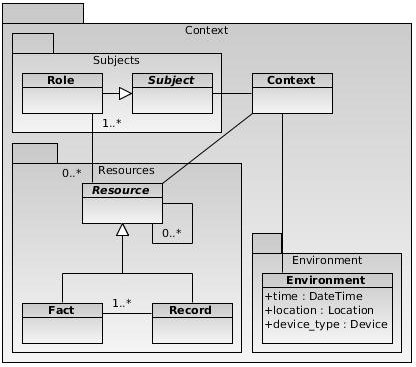
\includegraphics[width = 6cm]{UMOntology}
\end{figure}

\end{frame}

\section{Data Marketplace}
\begin{frame}
\frametitle{Data Marketplace}
A data marketplace, in this case, is a virtual environment in which data producers are able to profit by providing their information directly to various kinds of data consumers.  

\begin{figure}
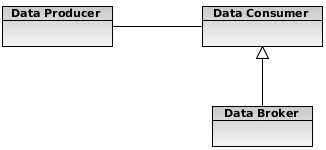
\includegraphics[width = 6cm]{roles}
\end{figure}
\pause

In General:
\begin{itemize}
\item \textit{Producers} produce data, \textit{Consumers} directly consume or redistribute data.  \textit{Producers} are holders of medical information, generally individual patients. \textit{Consumers} are institutions like research laboratories or pharmaceutical companies.
\end{itemize}

\end{frame}

\begin{frame}
\frametitle{Data Marketplace - Ontology}
\pause

\begin{figure}
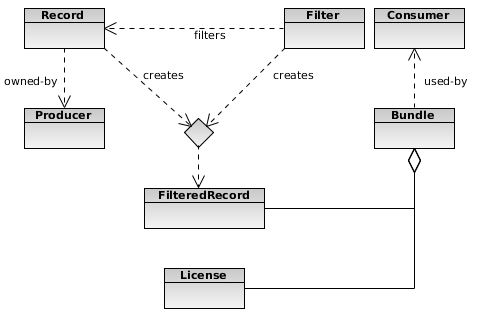
\includegraphics[width = 6cm]{ontology}
\end{figure}
\pause

\begin{itemize}
\item Use a combination of static and dynamic policy evaluation
\begin{itemize}
\item Static filtering of records pre-distribution is more efficient
\item Dynamic control allows for \textit{transitive attribution}, in which a consumer is appropriately credited for supplying data for products that are separated by more than one state
\end{itemize}
\pause

\item Note relationships to previous domain ontology
\begin{itemize}
\item Common elements include \textbf{Record, Role} entities
\end{itemize}
\end{itemize}

\end{frame}

\begin{frame}
\frametitle{Data Marketplace - System Attributes}

\begin{itemize}

\item \textit{Editability} Certain fields of that record should be editable by the owner.  Other fields must only be editable by specific medical providers.

\item \textit{Roles} Verifiable roles related to ownership of specific areas of a given record.

\item \textit{Auditability} Keeps a clear record of who edited what, what those specific changes were, how they were made, and when. 

\item \textit{Security} Use of modern security systems as much as possible to provide additional control over assets. 

\item \textit{Accessibility} Wide accessibility geographically, access to medical information from devices with a variety of form factors.

\item \textit{Performance} Core functionality must be high performance.

\item \textit{Flexibility} This system and the data it manages can be used in a wide variety of contexts.

\item \textit{Extensibility} It must provide programmatic interfaces.

\end{itemize}

\end{frame}

\begin{frame}
\frametitle{Data Marketplace - Logical View}

\begin{figure}
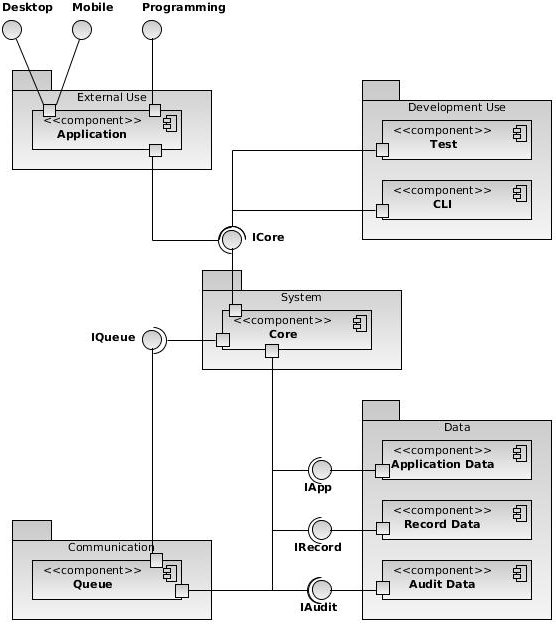
\includegraphics[width = 6cm]{HisbSystemArch}
\end{figure}

\end{frame}

\begin{frame}
\frametitle{Conclusions}

New Approach
\begin{itemize}
\item Protecting \textit{facts} rather than \textit{records} 
\end{itemize}

New Models
\begin{itemize}
\item More fine-grained control creates new opportunities around data management and use
\end{itemize}

Better Service
\begin{itemize}
\item New models provide new services, at the cost of new risks
\end{itemize}

\end{frame}

%\bibliographystyle{plain}
%\bibliography{drm}

\end{document}

